\beginsong{Es war an einem Sommertag}[wuw={Arno Clauss, 1973}, bo={136}, pfii={88}, pfiii={36}, gruen={176}, kssiv={26}, siru={78}]

\beginverse
\endverse
\centering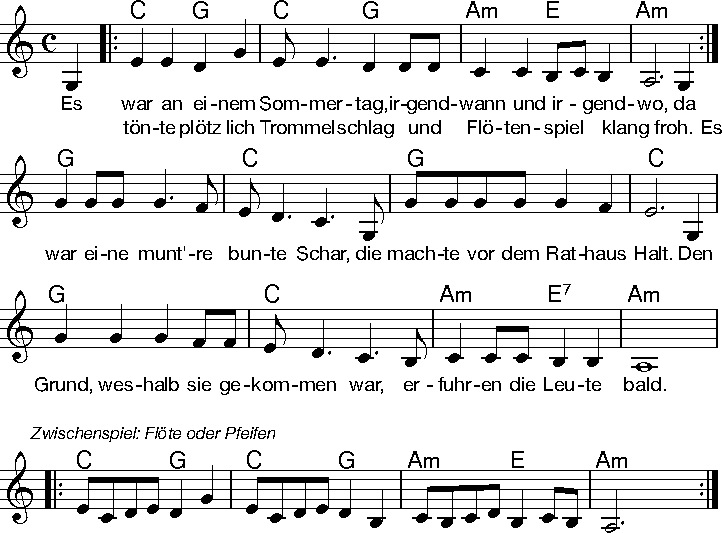
\includegraphics[width=1\textwidth]{Noten/Lied040.pdf}	

\beginverse
Ein \[C]Mann mit \[G]einem \[C]Feder\[G]hut rief: ''\[Am]Männer, \[E]hört mir \[Am]zu!
\[C]Ich ver\[G]sprech' euch \[C]Geld und Gut \[G]und \[Am]Ehre \[E]noch da\[Am]zu.
Der \[G]Kaiser braucht euch, \[C]reiht euch ein, denkt \[G]nicht an Weib und \[C]Haus!
Es \[G]muss ja nicht für \[C]lange sein, zieht \[Am]mit ins \[E]Feld hi\[Am]naus!''

{\nolyrics Zwischenspiel: \[C] \[G] \[C] \[G] \[Am] \[E] \[Am]}
\endverse

\beginverse
Im ^Wirtshaus ^war das ^Trinken ^frei, bezahlt ^mit des ^Kaisers ^Gold.
Und ^während ^dieser ^Zeche^rei trat ^mancher in des ^Kaisers ^Sold.\newpage
Gab ^seiner Braut den ^Abschiedskuss, ver^suchte als Soldat sein ^Glück,
Sah ^nicht des Werbers ^Pferdefuß und ^kam nicht ^mehr zu^rück.
{\nolyrics Zwischenspiel: \[C] \[G] \[C] \[G] \[Am] \[E] \[Am]}
\endverse

\beginverse
Mit ^Flöten^spiel und ^Trommel^schlag ging's ^früh am ^Morgen ^fort.
Die ^Schar ward ^größer, ^denn es ^lag am ^Weg noch ^mancher ^Ort.
Der ^Werber mit dem ^Federhut macht' ^sein Geschäft nicht ^schlecht,
ver^sprach noch vielen ^Geld und Gut, dem ^Kaiser ^dem war's ^recht.
{\nolyrics Zwischenspiel: \[C] \[G] \[C] \[G] \[Am] \[E] \[Am]}
\endverse

\beginverse
Die ^Jahre ^gingen ^in das ^Land und ^von der ^großen ^Schar
war ^keiner, ^der nach ^Hause ^fand, wie ^er ge^gangen ^war.
Der ^eine ließ sein ^Bein im Feld, blind ^kam ein and'rer ^an.
Die ^meisten hatte der ^Tod gefällt, der ^jede ^Schlacht ge^wann.
{\nolyrics Zwischenspiel: \[C] \[G] \[C] \[G] \[Am] \[E] \[Am]}
\endverse

\beginverse
Die ^letzten ^Tränen ^waren ^kaum ge^weint, da ^waren ^sie
auch ^schon ver^gessen, ^wie ein ^Traum; die ^Menschen ^lernen ^nie!
Und ^dann an einem ^Sommertag, irgend^wann und irgend^wo,
da ^tönte wieder ^Trommelschlag, und ^Flöten^spiel klang ^froh.
{\nolyrics Zwischenspiel: \[C] \[G] \[C] \[G] \[Am] \[E] \[Am]}
\endverse

\endsong
